\documentclass[12pt]{report}
%\documentclass{article}
\usepackage[utf8]{inputenc}
\usepackage{graphicx}
\graphicspath{.}
\usepackage{fullpage}

\title{CSCE 315 \\ Statement of Revision}
\author{Oscar Reyes,\\
	James Corder Guy,\\
	Oleksandr Sofishchenko}
\date{April 26, 2017}

\begin{document}
	
	\maketitle
	
	\newpage
	
	\begin{center}
		\title{\textbf{Aggie Spirit Bus Route App Statement of Revision}} \\
		
	\end{center}

	After our user study we found out that there are a couple of things that we could do to improve our website. At the moment, students like the way that the current Tamu bus website/app works. We would like to take the things that are good from the existing app and improve upon them.\\
	
	We believed that we had a very good interface, however, from the feedback we received we could change a couple of things. The first thing would be to reduce the amount of scrolling that we have on the website. Users did not like the fact that they had to scroll down to the map and also that the map did not support zooming in by pinching in or by using the scroll wheel. So that is one of the things we could change. Aside from the issue with scrolling, we received a good feedback on the looks of the website. At this point we were asked to add more functionality to the website. We aim towards tracking buses on the website, along with having the buttons for each route work.\\
	
	In order to implement the changes on the website we will need to do one of two things. The first thing will be to change the framework that we are using or changing the code of the current framework so it scrolls less. Maybe remove the title page and just add a smaller title that mentions this is a bus route app for Texas A\&M. We also need to add more code to make the map track the buses. Furthermore we need to overlay the routes on the google map and if possible track if buses are late in their route. We would also have to figure out a way to determine how much more time it would take for a bus to get to a specific stop.\\
	
	By the end of the project, we might aim towards the website looking like the following two sketches. \\
	
	\begin{figure}[h]
		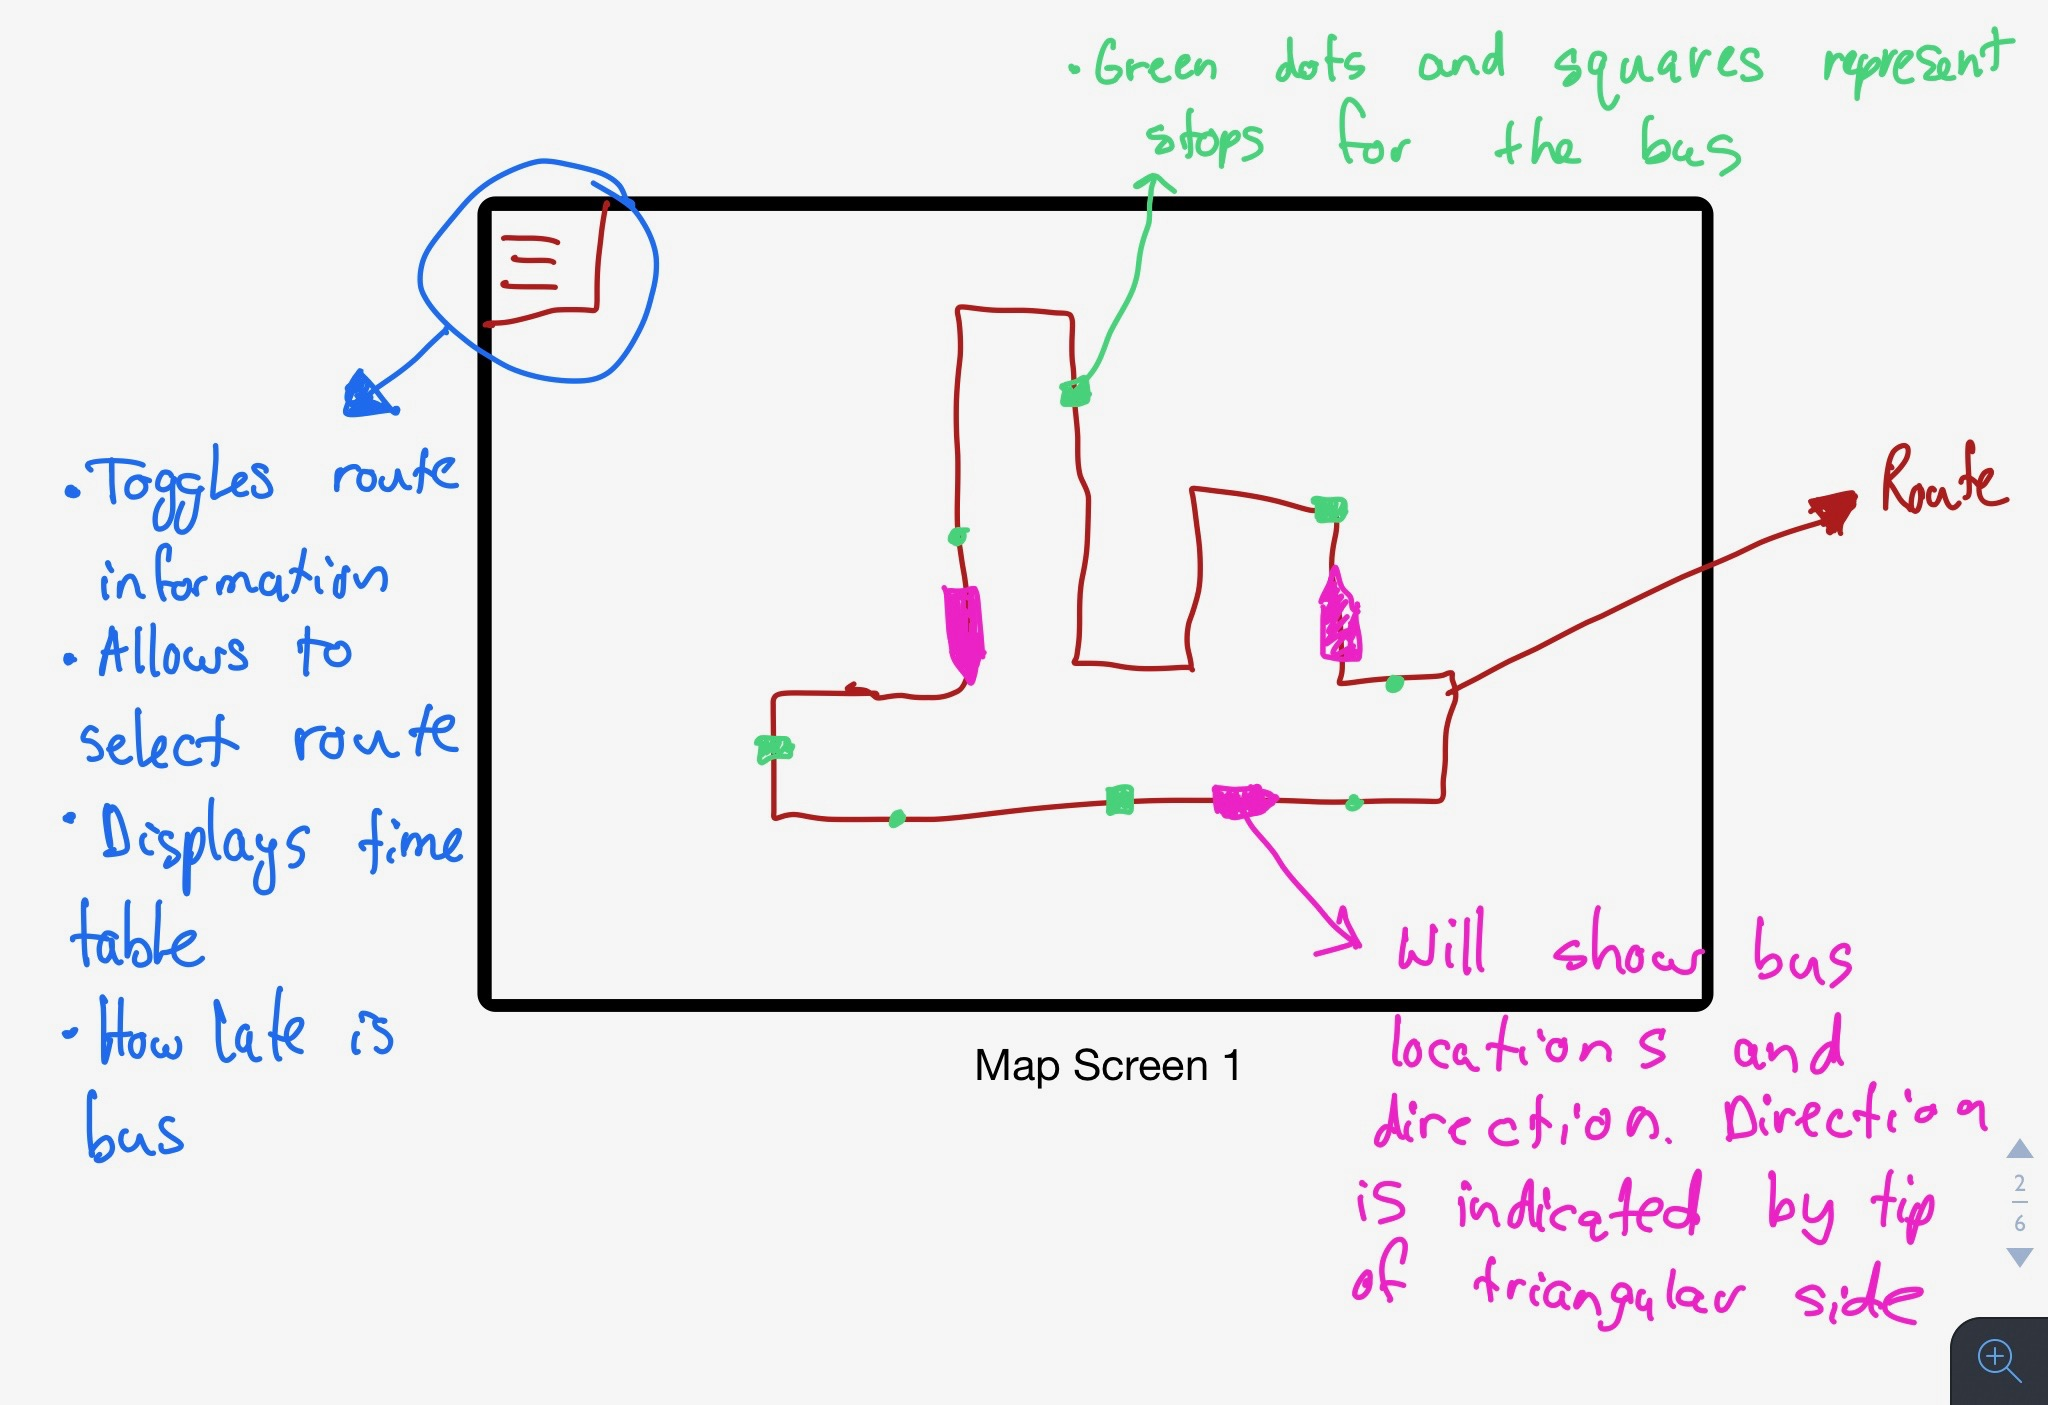
\includegraphics[scale=0.15]{MapScreen1}
		\centering
	\end{figure}
	\newpage
	
	
	\begin{figure}[h]
		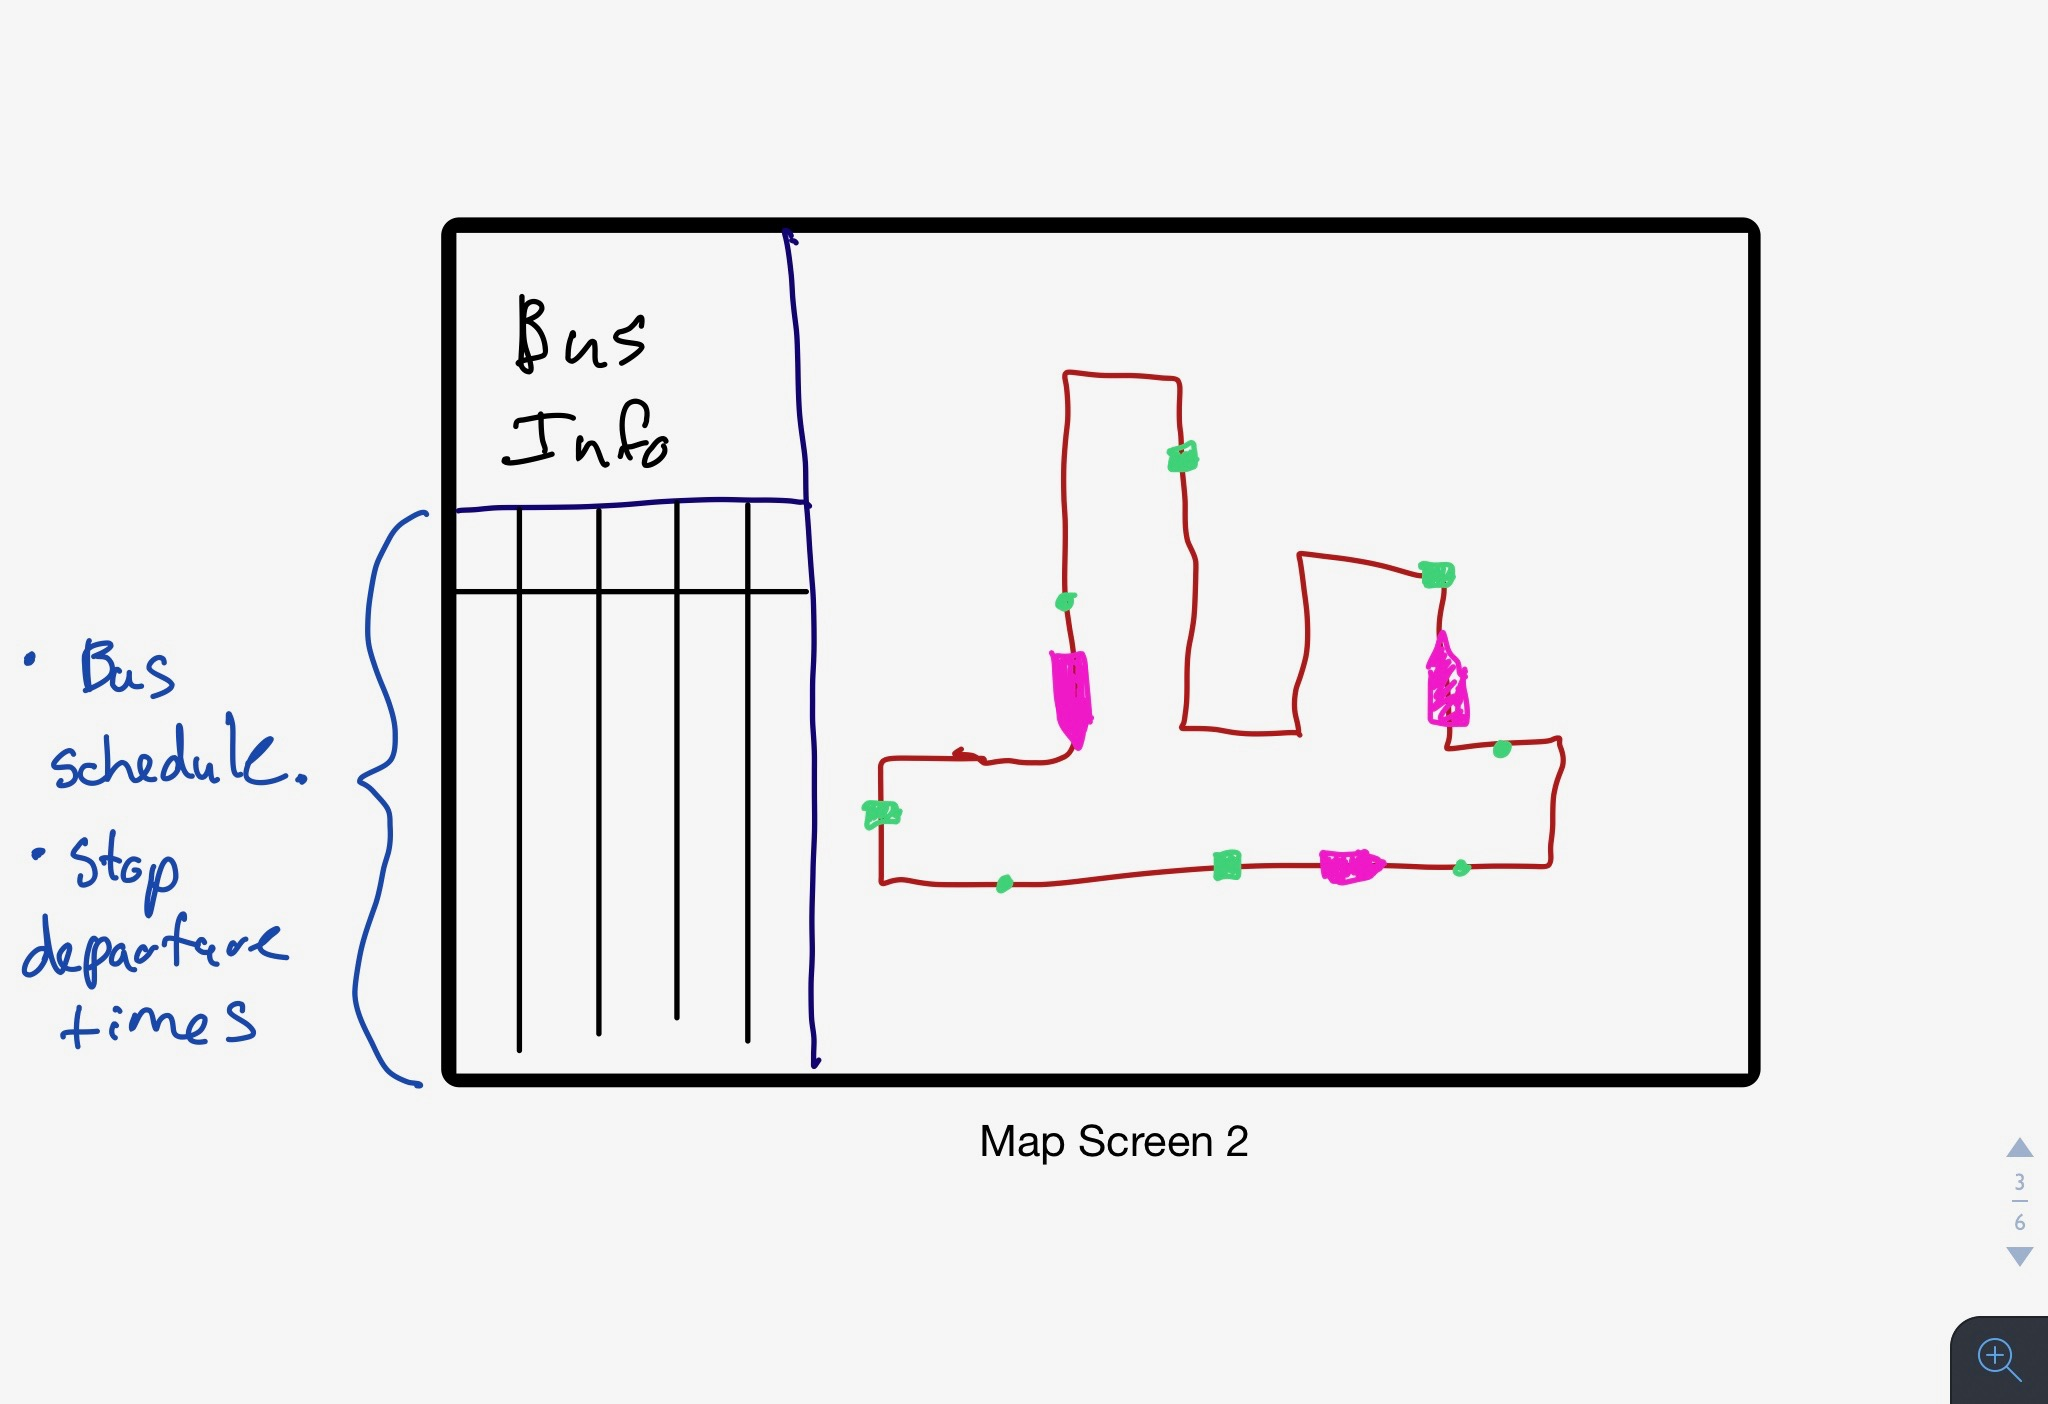
\includegraphics[scale=0.15]{MapScreen2}
		\centering
	\end{figure}
	
	These are the same sketches as the ones in the prototype, however, this time the title page will probably be gone and we will leave a user interface that is simpler and more to the point.\\

\end{document}